\documentclass[10pt,letterpaper]{article}
\usepackage[margin=0.85in,headheight=15pt]{geometry}
\usepackage[T1]{fontenc}
\usepackage{microtype,booktabs,array,longtable,graphicx,tikz,xcolor,hyperref,fancyhdr,caption,enumitem}
\usetikzlibrary{arrows.meta,positioning,fit}
\definecolor{navy}{HTML}{15344B}
\definecolor{teal}{HTML}{087E8B}
\hypersetup{colorlinks=true,urlcolor=teal,linkcolor=navy,pdftitle={LLM Adaptation Comparison: Weeks 8--9 Research Progress Update},pdfauthor={Somama Siddiqui}}
\captionsetup{font=small,labelfont=bf}
\setlength{\parskip}{0.35em}
\setlength{\parindent}{0pt}
\setlist[itemize]{topsep=2pt,itemsep=2pt,leftmargin=1.4em}
\pagestyle{fancy}\fancyhf{}
\fancyhead[L]{\small Senior Seminar I --- Research Progress Update}
\fancyhead[R]{\small Weeks 8--9}\fancyfoot[C]{\thepage}
\renewcommand{\headrulewidth}{0.4pt}
\newcolumntype{P}[1]{>{\raggedright\arraybackslash}p{#1}}
\title{\vspace{-1.1em}\textbf{A Comparative Evaluation of Fine-Tuning, Few-Shot Prompting, and Retrieval-Augmented Generation for Domain-Specific Question Answering with Small Language Models}\\[0.4em]\large Research Progress Update: Weeks 8--9}
\author{Somama Siddiqui\\Senior Seminar I \quad Instructor: Dr. Ning Zhang}
\date{October 19, 2026}
\begin{document}
\maketitle
\begin{abstract}
This report extends the Weeks 1--7 midterm study with completed GPU baselines and Version-1 low-rank adaptation training. All Colab conditions use Qwen~2.5~3B Instruct with the same NF4 inference backend on a Tesla T4. The retained runs contain 88 generated answers and 143 scoring rows over 11 synthetic policy facts. After a documented answer audit, both retrieval-augmented generation (RAG) methods score 10/11 with original knowledge and 11/11 after refreshing the source. Few-shot prompting scores 10/11 in both matching-version conditions. Version-1 LoRA scores 5/11 against original truth and 4/11 against updated truth. Training completed 20 epochs in 124.21 seconds, with 3.36~GiB peak allocated CUDA memory. These measurements complete the Week-9 initial and stale evaluation milestone. Continued training on Version~2 remains a Week-10 task. The small dataset, overlapping adaptation/evaluation facts, and single retained evaluation per condition limit generalization.
\end{abstract}
\textbf{Keywords:} factual staleness; retrieval-augmented generation; few-shot prompting; QLoRA; small language models.

\section{Project Overview}
The project investigates how a question-answering system acquires and refreshes domain facts using RAG, few-shot prompting, or low-rank fine-tuning. The fictional Nimbus Cloud Storage handbook has two versions: six evaluated facts change and five remain stable. The research question concerns factual accuracy, response latency, and computational demands before and after a policy update.

The intended final product is a reproducible comparison with source code, raw responses, measured results, architecture diagrams, and failure analysis. The Weeks 1--7 report established the dataset, local Llama/Ollama experiments, evaluation pipeline, and CUDA training implementation. This update reports the additional work completed for Weeks~8--9; the earlier midterm remains the historical record for the first seven weeks. Project completion remains targeted for \textbf{Week~11}.

\clearpage
\section{Work Completed: Weeks 8--9}
\subsection{Week 8: model access and comparable GPU baselines}
Hugging Face authentication succeeded, but the planned Llama~3.2~3B checkpoint download was denied for the project account. The Colab study therefore moved to the accessible \path{Qwen/Qwen2.5-3B-Instruct} checkpoint. Every Colab method uses this same base model. The local Llama pilot remains separate because changing the model, hardware, and backend prevents a controlled comparison between the two environments.

TF-IDF RAG, MiniLM embedding RAG, 13-example few-shot prompting, and a zero-shot control were run through the Hugging Face NF4 backend on a Tesla T4. RAG and few-shot were evaluated with both handbook versions. Zero-shot received no handbook information. The run saved 77 answers and 121 scoring rows, including original, stale, and refreshed conditions. The implementation uses Python, PyTorch, Transformers, sentence-transformers, scikit-learn, and JSON evidence files.

\begin{figure}[htbp]\centering
\resizebox{\linewidth}{!}{%
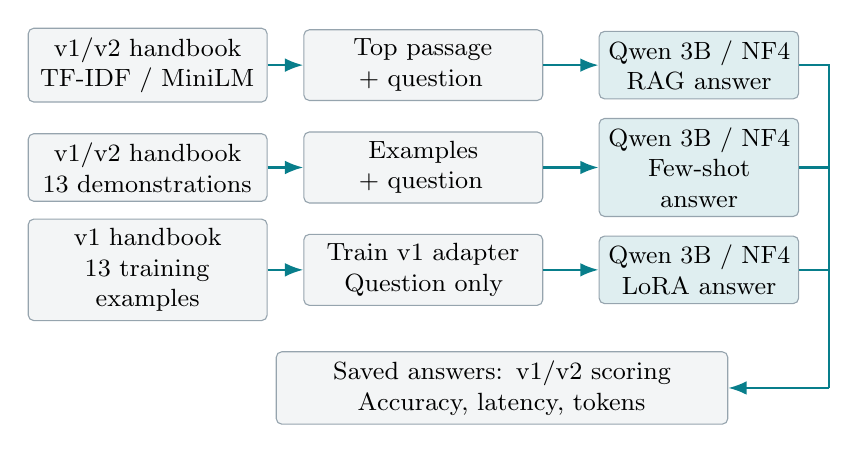
\begin{tikzpicture}[>=Latex,
 box/.style={draw=navy!45,rounded corners=2pt,fill=navy!5,align=center,text width=2.8cm,minimum height=0.85cm,font=\small},
 answerbox/.style={box,fill=teal!13,text width=2.3cm}]
\node[box] (r) at (0,2.5) {v1/v2 handbook\\TF-IDF / MiniLM};
\node[box] (f) at (0,1.2) {v1/v2 handbook\\13 demonstrations};
\node[box] (l) at (0,-0.1) {v1 handbook\\13 training examples};
\node[box] (rp) at (3.5,2.5) {Top passage + question};
\node[box] (fp) at (3.5,1.2) {Examples + question};
\node[box] (lp) at (3.5,-0.1) {Train v1 adapter\\Question only};
\node[answerbox] (rm) at (7,2.5) {Qwen 3B / NF4\\RAG answer};
\node[answerbox] (fm) at (7,1.2) {Qwen 3B / NF4\\Few-shot answer};
\node[answerbox] (lm) at (7,-0.1) {Qwen 3B / NF4\\LoRA answer};
\node[box,text width=5.5cm] (e) at (4.5,-1.6) {Saved answers: v1/v2 scoring\\Accuracy, latency, tokens};
\foreach \a/\b in {r/rp,rp/rm,f/fp,fp/fm,l/lp,lp/lm}{\draw[->,teal,thick] (\a)--(\b);}
\draw[teal,thick] (rm.east)--(8.65,2.5)--(8.65,-1.6);
\draw[teal,thick] (fm.east)--(8.65,1.2);
\draw[teal,thick] (lm.east)--(8.65,-0.1);
\draw[->,teal,thick] (8.65,-1.6)--(e.east);
\end{tikzpicture}}
\caption{Completed Colab architecture. Zero-shot uses the same base model with only the question and system prompt. Version-2 LoRA continued training is the remaining update path.}
\label{fig:architecture}
\end{figure}

\subsection{Week 9: Version-1 QLoRA training and evaluation}
The adapter was trained on 13 independently worded, handbook-derived examples. The 11 evaluation question strings were held out; their underlying facts deliberately overlap with training. Completion-only labels exclude prompt tokens from the loss. Training used 4-bit NF4 base weights with double quantization, rank-16 adapters on \texttt{q\_proj}/\texttt{v\_proj}, and a fixed 20-epoch budget. The tokenizer/masking preflight validated all 13 examples.

Training completed and saved adapter weights, tokenizer files, and measurement metadata. The adapter then generated 11 answers without supplied policy passages; those answers were scored against both truth versions, producing 22 rows. The retained evaluation is a rerun of that same adapter, not a second training trial. Ten repository tests pass, and saved result counts, summaries, source hashes, and original Colab file checksums were verified.

\clearpage
\section{Evidence of Progress}
\subsection{Accuracy and response to changed facts}
Table~\ref{tab:accuracy} uses the audited baseline file and the unchanged LoRA evaluation scores. Original means v1 knowledge against v1 truth; stale means the \emph{same v1 answers} against v2 truth; refreshed means v2 knowledge against v2 truth. Counts use 11 evaluated facts, not the larger number of scoring rows.

\begin{table}[htbp]\centering\small
\caption{Audited generated-answer accuracy. Each cell shows total correct, followed by stable/changed counts in parentheses.}\label{tab:accuracy}
\begin{tabular}{lccc}\toprule
Method & Original & Stale & Refreshed\\\midrule
TF-IDF RAG & 10/11 (5/5; 5/6) & 6/11 (5/5; 1/6) & 11/11 (5/5; 6/6)\\
Embedding RAG & 10/11 (5/5; 5/6) & 6/11 (5/5; 1/6) & 11/11 (5/5; 6/6)\\
Few-shot & 10/11 (5/5; 5/6) & 5/11 (5/5; 0/6) & 10/11 (5/5; 5/6)\\
Zero-shot & 1/11 (1/5; 0/6) & 1/11 (1/5; 0/6) & Not applicable\\
LoRA v1 & 5/11 (3/5; 2/6) & 4/11 (3/5; 1/6) & Pending\\\bottomrule
\end{tabular}
\end{table}

Both RAG methods incorrectly answer ``Yes'' to the v1 question about mandatory 2FA for standard accounts. That error coincidentally matches v2 truth; it does not demonstrate knowledge refresh. After re-indexing, both RAG methods answer all six changed facts correctly. Few-shot v2 still gives a 30-day refund window instead of 45 days. LoRA acquires some facts but makes errors on VPN timeout, refund processing, password resets, priority support, and Basic Plan capacity. Its v2 2FA match also includes an unsupported SMS requirement. Appendix~\ref{app:audit} explains scoring and examples.

\subsection{Measured runtime, token use, and training cost}
\begin{table}[htbp]\centering\small
\caption{Colab inference means over 11 generated answers per condition. Stale rescoring does not create additional latency observations.}\label{tab:latency}
\begin{tabular}{lrrr}\toprule
Method / knowledge & End-to-end seconds & Prompt tokens & Output tokens\\\midrule
TF-IDF RAG / v1 & 0.422 & 97.1 & 6.2\\
TF-IDF RAG / v2 & 0.416 & 97.9 & 6.2\\
Embedding RAG / v1 & 0.427 & 97.1 & 6.2\\
Embedding RAG / v2 & 0.438 & 97.9 & 6.2\\
Few-shot / v1 & 1.313 & 643.5 & 16.8\\
Few-shot / v2 & 1.370 & 652.5 & 17.5\\
Zero-shot / none & 0.312 & 66.5 & 4.7\\
LoRA / v1 & 2.339 & 66.5 & 28.6\\\bottomrule
\end{tabular}
\end{table}

Training took \textbf{124.21 seconds} around the training call; the Trainer's internal runtime was 123.72 seconds. Peak allocated CUDA memory was \textbf{3,612,005,888 bytes (3.36~GiB)} and average training loss was \textbf{0.8343}. Allocated tensor memory is not total device memory. Training time excludes initial base-model loading and adapter export. Inference excludes model loading and the warm-up generation; index setup is stored separately. All inference conditions use NF4 without double quantization, including adapter evaluation.

Longer LoRA outputs contribute to its larger mean latency; these timings do not isolate adapter overhead. Fixed condition order, one retained run per condition, and unequal context/output lengths limit efficiency comparisons. Energy and dollar cost were not measured.

\clearpage
\section{Progress Compared with the Recorded Plan}
The original approved proposal was not available in the supplied project records. Progress is therefore compared with the explicit Week~8--11 plan in the earlier midterm report, rather than asserting compliance with unverified original deadlines.

\begin{table}[htbp]\centering\small
\caption{Status against the midterm completion plan.}
\begin{tabular}{P{0.18\linewidth}P{0.45\linewidth}P{0.27\linewidth}}\toprule
Milestone & Recorded objective & Current status\\\midrule
Week 8 & Resolve model access and run comparable Colab baselines. & Complete using Qwen 3B.\\
Weeks 9--10 & Train v1, evaluate original/stale answers, then update on v2. & v1 complete; v2 remains.\\
Week 11 & Finalize audits, analysis, code, report, and demonstration. & Initial audit complete; final synthesis remains.\\\bottomrule
\end{tabular}
\end{table}

The research question and controlled dataset remain unchanged. The principal adjustment is the Colab base-model substitution. Within-Colab consistency was preserved by running every method with Qwen; local Llama measurements are not pooled with these results. The completed Week-9 milestone is consistent with the recorded plan. Meeting the Week-11 finish target still depends on the v2 adapter experiment and final analysis.

\section{Challenges and Solutions}
\subsection{Model access and limited local compute}
The 8~GiB Mac supported the earlier quantized local pilot but was not the CUDA training environment. Colab provided the Tesla T4. Successful account login did not confer permission to download the gated Llama model. Using the public Qwen checkpoint resolved the execution obstacle, while documenting the substitution preserved the distinction between the earlier local pilot and the GPU comparison.

\subsection{Scoring paraphrases and account scope}
The automatic scorer rejected zero-shot ``Daily'' because it expected numeric units. It also accepted a few-shot stale 2FA answer that qualified the requirement to accounts with administrative privileges. The answer audit accepted the daily-backup paraphrase under both truths and rejected the qualified 2FA response for the all-standard-account requirement. Three row-level overrides are stored in a separate audited JSON, with explanations and a hash of the original file. Raw outputs and automatic scores remain available. This assistant-assisted audit was neither independent nor blinded.

\subsection{Training success versus factual acquisition}
Successful completion of training did not yield uniformly correct answers: the v1 adapter scored 5/11, and some responses introduced unsupported details. The fixed training budget was retained rather than tuned against the evaluation answers. These failures are part of the measured outcome. Determining how continued v2 training affects both changed and stable facts remains unresolved.

\subsection{Transferring evidence from an ephemeral runtime}
Colab browser downloads failed. Text result files were recovered through the file editor, saved in GitHub, and checked against the original SHA-256 fingerprints. Adapter weights were archived in the runtime but were not transferred outside it. Evidence-file preservation is resolved; durable checkpoint backup remains an outstanding handoff task. The recorded adapter hash can identify a recovered checkpoint, but the hash alone cannot reconstruct it.

\clearpage
\section{Current Project Status}
The project now has a completed same-base-model comparison of RAG, few-shot prompting, zero-shot control, and Version-1 LoRA under the original and stale truth conditions. Refreshed RAG and few-shot conditions are also complete. The retained Colab evidence comprises \textbf{88 generated answers and 143 scoring rows}: 77/121 for baselines and 11/22 for the adapter. These are repeated evaluations of the same 11 policy facts, not 143 independent observations.

The code and results are on branch \path{codex/midterm-experiments} in the \href{https://github.com/Somama12/llm-adaptation-comparison}{project GitHub repository}. The results/status snapshot was pushed as commit \texttt{5b8bbd6}; the execution code was \texttt{a7d60e7}. This report adds the narrative and figures around that evidence. Appendix~\ref{app:artifacts} maps claims to the saved files.

\subsection{What is complete and what remains incomplete}
The Week-8 baseline and Week-9 v1 training/evaluation objectives are complete. Version-2 LoRA continued training, updated-adapter evaluation, and the final three-way recovery analysis remain incomplete. No v2 LoRA accuracy or training-time measurement is claimed. The prior notebook supports this next experiment, but prepared code is not evidence that it ran.

At the end of the recorded session, the v1 adapter was stored at \path{/content/llm-adaptation-comparison/artifacts/lora-v1} and a backup ZIP was created at \path{/content/week9_adapter_backup.zip}. Neither checkpoint was verified outside Colab. Runtime availability has not been rechecked for this report. If the session is lost, the fixed v1 recipe must be rerun before the Week-10 continuation; exact weight reproducibility should be verified rather than assumed.

\subsection{Limits on interpretation}
The corpus is synthetic and small. Training and few-shot examples cover the same facts as evaluation, while holding out question wording. This tests acquisition and retention of known facts rather than generalization to new domains. Few-shot uses all 13 demonstrations, whereas RAG supplies one passage. One retained deterministic evaluation per condition does not quantify variation across seeds or repeated training runs. Core-fact scoring can accept an answer that also contains unsupported claims, so numeric accuracy must be read alongside the failure analysis.

\section{Plan for Weeks 10--11}
\begin{table}[htbp]\centering\small
\caption{Remaining work toward the Week-11 completion target.}
\begin{tabular}{P{0.14\linewidth}P{0.47\linewidth}P{0.29\linewidth}}\toprule
Period & Task & Required evidence\\\midrule
Week 10 & Recover or reproduce v1; continue the adapter on v2 using the fixed recipe; evaluate against v2 truth. & Saved adapter, raw answers, training time, and peak CUDA allocation.\\
Week 10 & Compare recovery on six changed facts and retention on five stable facts; inspect unsupported claims. & Updated comparison table and documented answer audit.\\
Week 11 & Finalize interpretation, reproduction instructions, research report, and demonstration. & Complete repository, final PDF, and project presentation.\\\bottomrule
\end{tabular}
\end{table}

The next experiment should preserve both adapters and use a distinct v2 output file. Any later hyperparameter exploration should be labeled exploratory and use a separate validation design. The existing v1 result should remain available as the fixed-budget baseline.

\clearpage
\appendix
\section{Evaluation Facts and Scoring Audit}\label{app:audit}
\begin{table}[htbp]\centering\small
\caption{The 11 evaluation facts. Labels abbreviate the IDs in \texttt{eval/qa\_pairs.json}; question descriptions are shortened.}
\begin{tabular}{lP{0.41\linewidth}P{0.20\linewidth}P{0.20\linewidth}}\toprule
ID & Fact & v1 truth & v2 truth\\\midrule
S1 & VPN session timeout & 8 hours & 8 hours\\
S2 & Refund processing & 5 business days & 5 business days\\
S3 & Paid-tier backup frequency & Every 24 hours & Every 24 hours\\
S4 & Ticket escalation & 48 hours & 48 hours\\
S5 & Pro Plan storage and price & 2 TB; \$12.99/mo & 2 TB; \$12.99/mo\\\midrule
C1 & Password-reset interval & 90 days & 60 days\\
C2 & Standard-account 2FA & Optional & Mandatory\\
C3 & Full-refund request window & 30 days & 45 days\\
C4 & Backup retention after deletion & 30 days & 90 days\\
C5 & Priority-tier initial response & 4 hours & 2 hours\\
C6 & Basic Plan capacity & 100 GB & 150 GB\\\bottomrule
\end{tabular}
\end{table}

\subsection{Documented row-level corrections}
\begin{table}[htbp]\centering\small
\caption{Audit overrides; the generated answers were not regenerated or edited.}
\begin{tabular}{P{0.25\linewidth}P{0.24\linewidth}P{0.41\linewidth}}\toprule
Record & Decision change & Reason\\\midrule
Zero-shot S3, v1 truth & Incorrect $\rightarrow$ correct & ``Daily'' expresses the expected 24-hour frequency.\\
Zero-shot S3, v2 truth & Incorrect $\rightarrow$ correct & The stable fact and same response apply to v2.\\
Few-shot v1 C2, v2 truth & Correct $\rightarrow$ incorrect & ``With administrative privileges'' restricts the account scope; it does not support the general standard-account requirement.\\\bottomrule
\end{tabular}
\end{table}

These corrections change zero-shot from 0/11 to 1/11 under either truth, and stale few-shot from 6/11 to 5/11. All other baseline decisions and all LoRA decisions are unchanged. The audit inspected 88 generated records and their relevant truth conditions. It was an assistant review, not a separate human annotation study.

\subsection{Representative LoRA errors}
LoRA's VPN response invents a five-minute timeout for unauthenticated sessions and no expiry for authenticated sessions, instead of eight hours. Its refund-processing response gives four business days instead of five. Its password-reset response says 12 months instead of 90 days, and its Basic Plan answer gives 2~GB instead of 100~GB. These descriptions summarize the saved responses; exact text is in \path{results/lora_v1.json}.

The 2FA answer states that all standard accounts must use SMS-based authentication and continues in another language. It receives a v2 core-fact match for stating that 2FA is required, while the SMS restriction and extra continuation remain unsupported. This distinction prevents a single accuracy score from concealing response-quality failures. Conversely, correctly recalled Pro Plan specifications and backup/escalation facts show that the adapter did acquire some task information.

\clearpage
\section{Protocol, Environment, and Evidence Map}\label{app:artifacts}
\subsection{Reproducibility settings}
\begin{table}[htbp]\centering\small
\caption{Recorded training and evaluation configuration.}
\begin{tabular}{P{0.33\linewidth}P{0.57\linewidth}}\toprule
Component & Setting\\\midrule
Base model and accelerator & Qwen/Qwen2.5-3B-Instruct; Tesla T4\\
Training quantization & NF4; double quantization enabled; FP16 compute\\
Adapter & Rank 16; alpha 32; dropout 0.05; query/value projections\\
Training schedule & 20 epochs; seed 42; learning rate $2\times10^{-4}$\\
Batch and objective & Batch 1; accumulation 4; completion-only labels; 13 examples\\
Inference & NF4 without double quantization; deterministic decoding; maximum 96 new tokens; one untimed warm-up\\
Runtime & Python 3.13.15; torch 2.11.0+cu130; Transformers 4.57.6\\
Training libraries & PEFT 0.21.1; Accelerate 1.15.0; bitsandbytes 0.50.2; huggingface-hub 0.36.2\\\bottomrule
\end{tabular}
\end{table}

The saved baseline and adapter runs record matching hashes for the experiment, retrieval, and training source files. The retained adapter evaluation has a dirty-working-tree flag that includes generated result files. It replaced an earlier evaluation of the same adapter; that earlier run is not retained or counted as a replication. The original result-file hashes match the Colab export after removal of a transfer-added final newline.

\subsection{Evidence map}
\begin{table}[htbp]\centering\small
\caption{Repository artifacts supporting this update.}
\begin{tabular}{P{0.48\linewidth}P{0.42\linewidth}}\toprule
Path & Evidence\\\midrule
\path{results/colab_baselines.json} & Original 77 answers and 121 automatic scoring rows.\\
\path{results/colab_baselines_audited.json} & Audited baseline, source hash, and three explicit overrides.\\
\path{results/lora_v1.json} & Eleven adapter answers and 22 scoring rows.\\
\path{results/training_v1.json} & Actual duration, GPU allocation, epochs, and average loss.\\
\path{results/week9_provenance.json} & Package versions and result/adapter SHA-256 fingerprints.\\
\path{docs/week8_9_results.md} & Detailed per-group accuracy and latency summaries.\\
\path{finetune/train.py} & Fixed-budget training and metadata collection.\\
\path{notebooks/colab_lora.ipynb} & GPU baseline, training, evaluation, and update workflow.\\\bottomrule
\end{tabular}
\end{table}

\subsection{Core Version-1 reproduction commands}
Run inside the repository with the training dependencies installed and a CUDA GPU. Use new output paths to preserve the recorded trial.
\begin{small}\begin{verbatim}
python -m finetune.train --model Qwen/Qwen2.5-3B-Instruct \
  --version v1 --output artifacts/lora-v1-reproduction
python -m experiments.run --backend hf \
  --model Qwen/Qwen2.5-3B-Instruct --methods lora \
  --adapter artifacts/lora-v1-reproduction \
  --knowledge-versions v1 --output results/lora_v1_reproduction.json
\end{verbatim}\end{small}
\end{document}
